\chapter{Grundlagen}
\label{kap2}

\section{Laufroboter}

Dieser Abschnitt stellt die für diese Arbeit relevanten Laufroboter vor. Dies ist zum einen der \emph{Lauron III}, für den der vorliegende Laufplaner entwickelt wurde; zum anderen ist dies der \emph{Akrobat}, für den der existierende Laufplaner migriert werden soll. Beide sind sich ziemlich ähnlich, jedoch sind die Unterschiede wichtig, um den Laufplaner auf den Akrobat zu migrieren. 

\subsection{Lauron}

Die erste Version des Lauron (Laufender Roboter Neuronal gesteuert) wurde 1994 am Forschungszentrum für Informatik (FZI) in Karlsruhe \autocite{fzi} entwickelt. Zunächst war es das Ziel Laufmuster durch neuronale Netze zu entwickeln und zu testen. Die zweite Version des Lauron verbessert die Sensorausstattung sowie die Mechanik des Laufroboters. Des Weiteren wurde das Steuerungsprinzip, das auf neuronalen Netzen basierte, durch die hierarichische MCA-Architektur \autocite{scholl2001modular} ausgetauscht. Für die dritte Version \emph{Lauron III}, siehe \autoref{kap2:lauron3}, existiert der vorliegende und zu übertragende Laufplaner in Form der 3D-Bibliothek OpenInventor \autocite{inventor}. Daher wird nun näher auf diese Version des Laufroboters sowie auf das grundlegende Konzept des Lauron als Nachahmung der indischen Stabheuschrecke eingegangen. Eine weitere Version des Laufroboters ist der \emph{Lauron IVb}, siehe \autoref{kap2:lauron4b}, welcher sich an der Hochschule Mannheim befindet. Die neuste Version des Laufroboters ist der \emph{Lauron V}.

Der Lauron basiert auf dem Vorbild der indischen Stabheuschrecke (Carausius morosus), die sehr gut erforscht ist. Dies gilt sowohl für den mechanischen Aufbau als auch für die Abläufe der Bewegungen des Roboters. Der Körper ist in drei Teile geteilt.
\begin{itemize}
  \item Kopf (Caput)
  \item Brust (Thorax)
  \item Hinterleib (Abdomen)
\end{itemize}

Die Brust ist wiederum in weitere drei Teile für jeweils ein Beinpaar unterteilt. Damit ergeben sich sechs Beine. Ein Bein besteht aus drei Segmenten:
\begin{itemize}
  \item Hüfte (Coxa)
  \item Oberschenkel (Femur)
  \item Unterschenkel (Tibia)
\end{itemize}

\begin{figure}[b!]
  \centering
  \begin{subfigure}[b]{.4\linewidth}
    \centering
    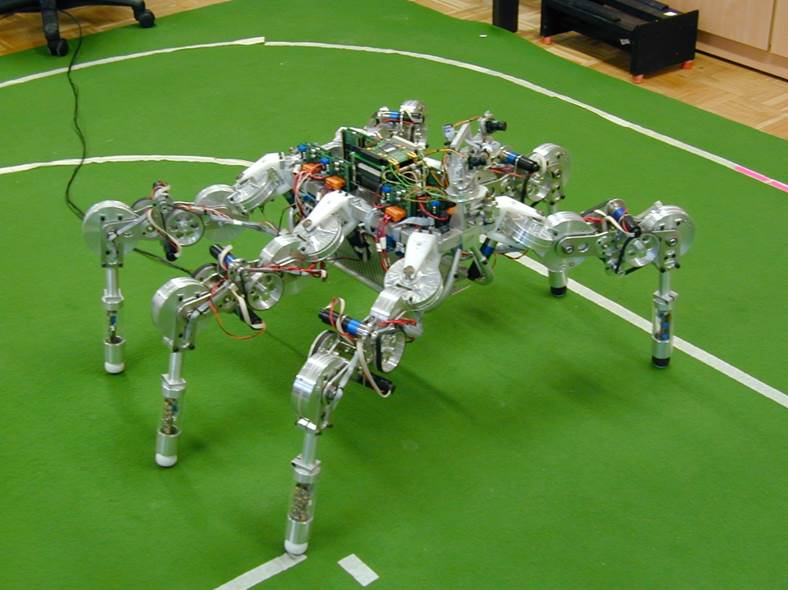
\includegraphics[width=6cm]{kapitel2/lauron3}
    \subcaption{Lauron III}\label{kap2:lauron3}
  \end{subfigure}%
  \qquad
  \begin{subfigure}[b]{.4\linewidth}
    \centering
    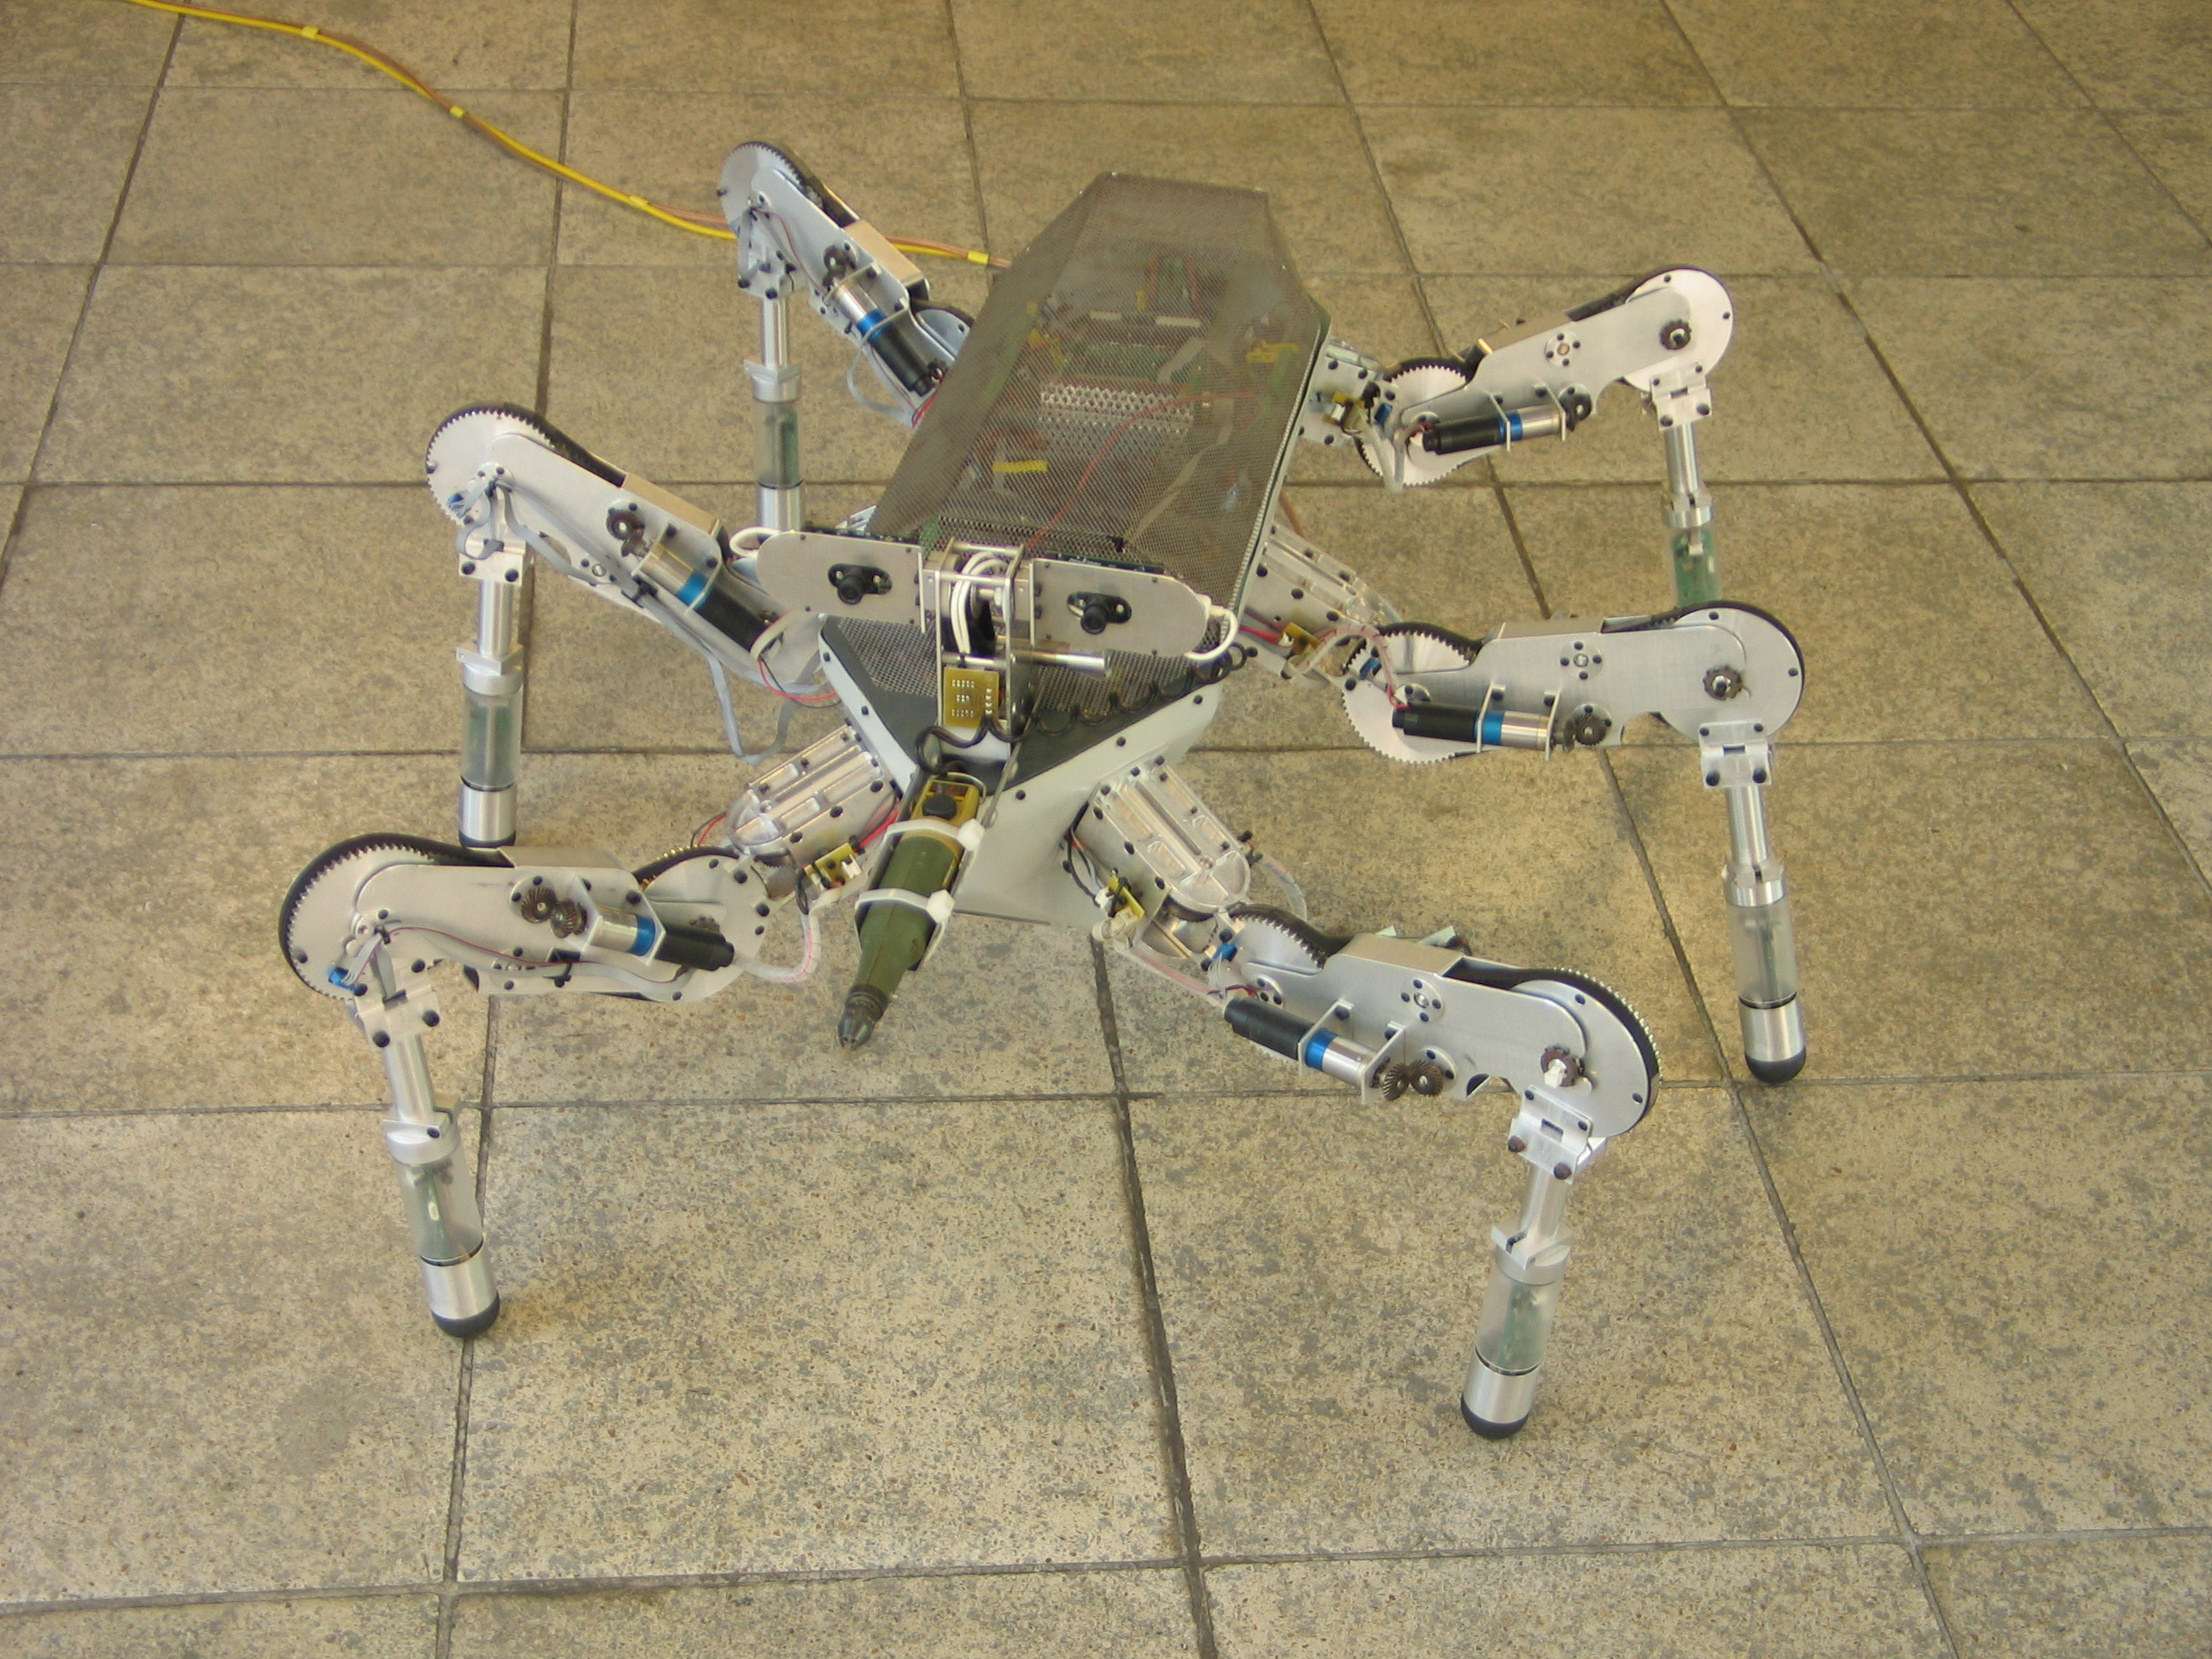
\includegraphics[width=6cm]{kapitel2/lauronivb}
    \subcaption{Lauron IVb}\label{kap2:lauron4b}
  \end{subfigure}\\
  \caption{Verschiedene Versionen des Lauron}
  \label{kap2lauron}
\end{figure}

Die Segmente sind durch die Gelenke Subcoxal $\alpha$, Coxa-Trochanter $\beta$ und Femur-Tibia $\gamma$ verbunden. Der Fuß jedes Beins wird Tarsus genannt. Das erste Gelenk Subcoxal besitzt zwei Freiheitsgrade, die weiteren Gelenke besitzen ein Freiheitsgrad. Damit ist für die indische Stabheuschrecke die minimale erforderliche Zahl an Freiheitsgraden erreicht, damit der Fuß beliebig im dreidimensionalen Raum gesetzt werden kann.

Unter anderem ist noch wichtig, dass der Kopf der indischen Stabheuschrecke zwei lange Fühler besitzt. Diese könnten in einem Roboter beispielsweise als Laserscanner oder Kamera modelliert werden, welche sich einen Überblick über die Gegend verschaffen können.

Der Körper des \emph{Lauron III} trägt die Microcontroller, die Recheneinheit, die Akkumulatoren sowie den Kamerakopf. An beiden Seiten des Körpers sind jeweils drei Beine angebracht. Der Roboter wiegt 16 Kilogramm und hat eine maximale Zuladung von etwa 15kg. Die Maximalgeschwindigkeit beträgt \SI{0.5}{\metre\per\second}. \autocite{gassmann2000} \autocite{troilo2007}

\subsection{Akrobat}

\begin{figure}[b!]
  \centering
  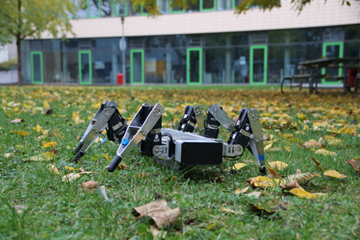
\includegraphics[height=8cm]{kapitel2/akrobat}
  \caption{Der Akrobat vor dem C-Gebäude der Hochschule Mannheim}
  \label{Kap2:akrobat}
\end{figure}

Auch der \emph{Akrobat} (\autoref{Kap2:akrobat}) ist der Form einer Stabheuschrecke nachempfunden und ähnelt in vielerlei Hinsicht dem Lauron.

Der Roboterkörper ist ungefähr 56 Millimeter hoch, 102 Millimeter breit und hat eine Seitenlänge von 62 Millimeter. Ebenfalls besitzt dieser sechs Beine mit je drei Segmenten. Diese haben die Längen 72 Millimeter, 97 Millimeter und 163 Millimeter, welche für kinematische Berechnungen von großer Bedeutung sind. Jedes Bein wiegt ungefähr 0,8 Kilogramm.

Jedes der Gelenke hat exakt einen Freiheitsgrad, sodass das gesamte Bein drei Freiheitsgrade hat. Wie auch beim Lauron ermöglicht dies die beliebige Positionierung im dreidimensionalen Raum. Die Gelenke sind mit dem Servomotor Dynamixel RX64 ausgestattet. Außerdem hat jedes Gelenk einen definierten Arbeitsbereich, welcher nicht unter- oder überschritten werden darf.
\begin{itemize}
  \item $\alpha$: -50$^\circ$ bis 50$^\circ$
  \item $\beta$: -106$^\circ$ bis 106$^\circ$
  \item $\gamma$: -135$^\circ$ bis 135$^\circ$
\end{itemize}  

Außerdem besitzt der Roboter am Kopf eine Kamera, welche aus zwei Freiheitsgraden besteht. Der Roboterkörper verfügt über genügend Freiraum für Batterien im mittleren Gehäuse. Im hinteren Gehäuse ist der Steuerrechner sowie die restliche Elektronik platziert.

Es handelt sich beim Rechner um den Einplatinencomputer Raspberry Pi (Modell B+) mit 521 MB Arbeitsspeicher und einem 700 MHz ARM 11 Prozessor. Der Raspberry Pi bietet vielfältige Anschlussmöglichkeiten: Wireless Local Area Network (WLAN), vier Universal Serial Bus (USB)-Anschlüsse ein Ethernet-Anschluss sowie einen High Definition Multimedia Interface (HDMI)-Anschluss. Über letzteren erfolgt die Visualisierung mittels eines externen Bildschirms. Es besteht die Möglichkeit das Gamepad F710 von Logitech per WLAN anzuschließen. Theoretisch sind auch andere Gamepads möglich, sofern diese im Quellcode konfiguriert wurden. \autocite{askerow2014}

\section{Robotik}

\subsection{Koordinatensysteme}
\subsection{Direkte Kinematik}

- Mit gegebener Stellung der Gelenke Position und Orientierung des Endeffektes zu berechnen
- Transformationsmatrix, die dann aufgelöst wird und berechnet werden kann

fellmann zitieren

\autocite{fellmann2007}

\subsection{Inverse Kinematik}

- Durch Position und Orientierung des Endeffektes mögliche Stellung der Gelenke zu berechnen (meist mehrere Lösungen)
- analytische Berechnung
- numerische Berechnung: lineare Annäherung durch Jacobi-Matrix

fellmann zitieren

\autocite{fellmann2007}

\subsection{Laufplanung}

statische Laufalgorithmen, reaktive, planende Laufalgorithmen like RandomSampling

\section{Frameworks}

Dieses Kapitel stellt die benötigten Frameworks für diese Arbeit dar. Das ist zum einen das \ac{ROS}, welches die Basis der Entwicklung darstellt. Zum anderen ist das Gazebo, welches als Physik-Engine und 3D-Visualisierung genutzt wird.

\subsection{Robot Operating System}

Für diese Arbeit ist der Aufbau und die Funktionsweise von \ac{ROS} von großer Bedeutung, da der Laufplaner auf diese Plattform migriert werden soll. Diese Themen werden in zahlreicher Literatur behandelt. \autocite{rosAnOpenSourceRobotOperatingSystem} \autocite{learningROSForRoboticsProgramming} \autocite{gentleIntroductionToROS}

Das \ac{ROS} ist ein Meta-Betriebssystem, welches primär auf der Linux Distribution Ubuntu und Debian verfügbar sind. Ebenfalls läuft \ac{ROS} auch unter Windows Services für Linux. Es existieren auch experimentelle Versionen wie beispielsweise für Mac OS X. Ein ROS-Release ist immer an eine \ac{LTS}-Version von Ubuntu  geknüpft. Das \ac{ROS} besteht aus vielen wichtigen und nützlichen Komponenten. Diese werden nun Schritt- für Schritt erklärt.

\subsubsection{Packages, Nodes und Stacks}

Sogenannte Packages bilden die Grundlage einer jeden \ac{ROS}-Entwicklung. In einem Paket werden alle nötigen Dateien gespeichert, die für das zu lösende Problem benötigt werden. Dies sind neben einem Manifest (package.xml), verschiedene Nodes, welche für die Berechnungen zuständig sind, Definitionen für Nachrichten und Services, damit die Nodes untereinander kommunizieren können sowie benötigte CMake-Konfigurationen, damit das Projekt erfolgreich gebaut werden kann. Nodes können in C++ oder Python programmiert werden. Theoretisch sinda auch andere Sprachen denkbar, allerdings haben sich diese beiden Varianten bewährt.

Eine Stufe über den Packages besteht die Möglichkeit der Organisation zusammengehöriger Packages in Stacks. Dies hat vor allem Vorteile hinsichtlich der Wiederverwendbarkeit und Erweiterbarkeit von Software. Möchte der Entwickler beispielsweise die Funktionalität einer Verbindung zu einem Bluetooth-Controller getrennt vom Ausführen der dazugehörigen Bewegung trennen, ist dies sinnvoll. Dann ließe sich leicht ein weiteres Package für einen anderen Controller entwickeln, ohne die bestehenden Packages zu beeinflussen.

\subsubsection{Kommunikation zwischen Nodes}

Die Kommunikation zwischen Nodes kann über Topics oder Services erfolgen.

Topics folgen dem Publisher-Subscriber Prinzip. Das bedeutet, dass eine Node Nachrichten veröffentlicht, während eine andere diesen Nachrichtenkanal verfolgt. Es können auch mehrere diesen Nachrichtenkanal verfolgen. Das Nachrichtenformat ist das msg-Format. Solche Formate werden nach Konvention im msg-Ordner abgespeichert.

Services folgen dem Client-Server-Prinzip. Hierbei handelt es sich um eine einmalige Abfrage einer Node. Der Client fragt eine Berechnung einmalig beim Server an.  Das Nachrichtenformat ist das srv-Format. Auch diese werden nach Konvention im msg-Ordner gespeichert.
    
Jede Nachricht beinhaltet einen sogenannten Header, der aus einer Identifikationsnummer, einem Zeitstempel sowie einr Frame-ID besteht.

\subsubsection{ROS-Master}

Vor jeder Ausführung einer Node in \ac{ROS} muss der sogenannte \ac{ROS}-Master gestartet werden. Dieser ist die zentrale Einheit im System, welche für jegliche Lookups sowie Namensregistrierungen der Nodes zuständig ist. Ohne den \ac{ROS}-Master ist keine Kommunikation zwischen Nodes möglich. Außerdem bietet dieser unter anderem noch die Möglichkeit \ac{ROS} auf verschiedenen Maschinen verteilen zu lassen. Die Konfiguration erfolg über Umgebungsvariablen im System, welche die IP-Adresse der Systeme beinhalten.

\subsubsection{Launch-Files}

Nodes können manuell über die Kommandozeile gestartet werden. Dies ist bei einer wachsenden Zahl an Nodes und Konfigurationen immer schwieriger, weshalb es sogenannte Launch-Files gibt. Diese bündeln gewisse Funktionalität, die ausführt werden sollen. \autoref{exampleLaunchFile} zeigt ein Beispiel dafür. Mit dem include-Befehl können weitere Launch-Files eingefügt werden. Auch dies trägt dazu bei, eine bessere Modularität zu erreichen. Mit dem node-Befehl wird eine Node aus einem Package gestartet. Launch-Files bieten viele weitere Möglichkeiten wie das Setzen von Parametern, welche innerhalb der Ausführung von Nodes genutzt werden können. Außerdem können Aufrufe von Nodes weiter konfiguriert werden. Beispielsweise kann mittels des output-Befehls gesteuert werden, wo die Konsolenausgaben ausgegeben werden. Der respawn-Befehl lässt eine Node neustarten, wenn sie abgestürzt ist. Der required-Befehl legt fest, dass nach Absturz diese Node die komplette Anwendung ebenfalls gestoppt werden soll.

\begin{lstlisting}[label={exampleLaunchFile}, language=Xml, caption={Beispiel eines Launch-Files}]
<launch>
  <include file="$(find hexapod)/launch/model.launch"/>
  
  <node name="akrobat" pkg="hexapod" type="akrobat" output="screen" respawn="false" required="true"></node>
</launch>
\end{lstlisting}
  
\subsubsection{Bag-Files}

Gerade in der Roboterentwicklung ist es oftmals nicht sinnvoll, Abläufe während der Entwicklung wiederholt auf dem Roboter ausführen zu müssen. Während in der Softwareentwicklung dies normalerweise kein Problem darstellt, kann der Roboter durch eine falsche Bewegung kaputt gehen oder auf lange Sicht abgenutzt werden. Daher bietet das \ac{ROS} die Möglichkeit alle Daten, die von Topics gesendet wurden mittels eines sogenannten Bags aufzunehmen und erneut abzuspielen. Dies lässt sich auch sinnvoll mit einer Simulation kombinieren. Bag-Aufnahmen oder Wiedergaben können sowohl über die Kommandozeile als auch in Launch-Files ausgeführt werden.

\subsubsection{Kommandozeilen-Tool}

Nahezu alle wichtigen \ac{ROS}-Dienste lassen sich über die Kommandozeile steuern. Jedes vorgestellte Konzept hat ein eigenes Interface, welches für eine unkomplizierte Interaktion sorgt:
\begin{itemize}
\item Nodes: rosrun
\item Topics: rostopic
\item Services: rosservice
\item Launch-Files: roslaunch
\item Bags: rosbag
\end{itemize}

Des Weiteren gibt es für einige Standardbefehle aus Linux Wrapper-Funktionen wie \glq ls\grq und \glq cd\grq, welche speziell für \ac{ROS} entwickelt wurden. Diese sind \glq rosls\grq und \glq roscd\grq, welche den \ac{ROS}-Ordner auflisten oder direkt in ein \ac{ROS}-Package wechseln.

\begin{figure}[t!]
  \centering
  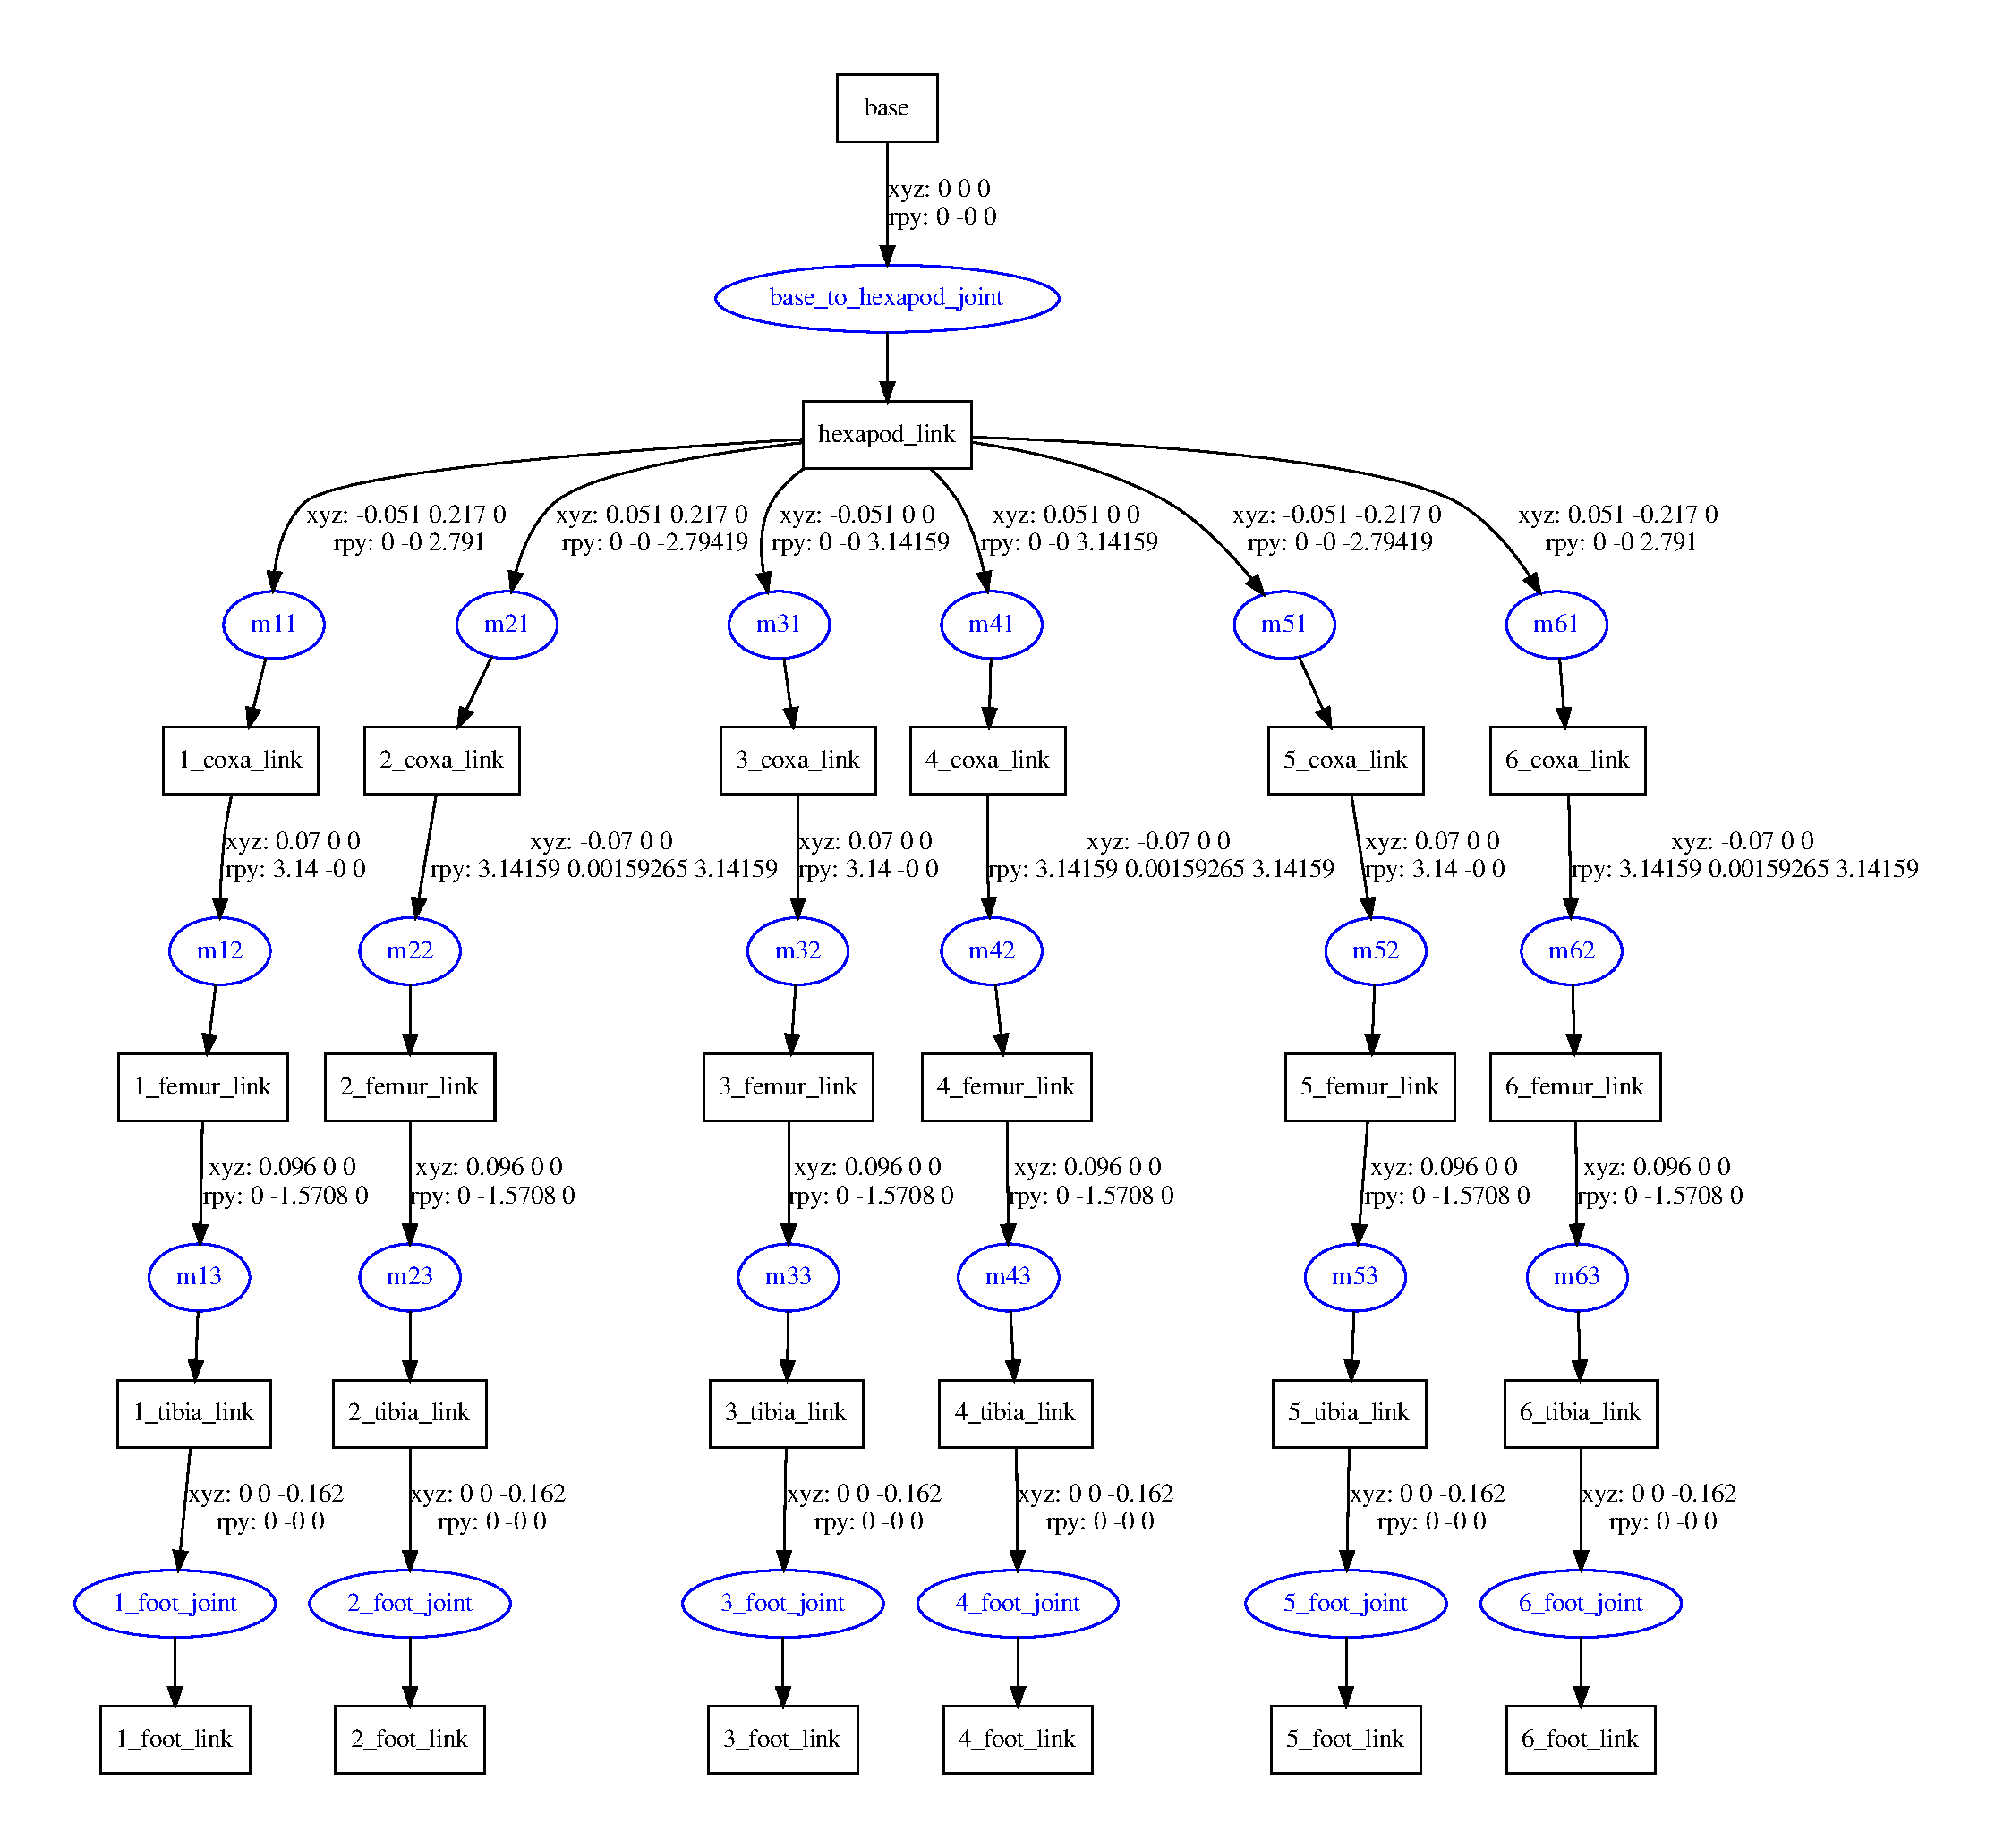
\includegraphics[height=8cm]{kapitel2/urdtographizakrobat}
  \caption{Darstellung des Transformationsbaums des Akrobats}
  \label{Kap2:urdtographizakrobat}
\end{figure}

\subsubsection{Robotermodell und tf-Framework}

Robotermodelle können in einem \ac{URDF} angegeben werden. Dieses Format beinhaltet jedes Segment und jedes Gelenk sowie deren Zusammenspiel. Dabei wird für jedes Segment die Visualisierung, die Massenträgheit sowie ein Kollissionsmodell angegeben. Die Visualisierung und die Kollission erfolgt beispielsweise über das Format \ac{STL}, aber auch, falls möglich, über einfache geometrische Objekte. Die Gelenke beinhalten den Verweis auf das Eltern- und auf das Kindelement sowie einen Arbeitsbereich. Eine Möglichkeit das \ac{URDF}-Format zu verbessern bieten \ac{Xacro}. \ac{Xacro} zielt vor allem darauf ab das Format lesbarer und kürzer zu gestalten. Über Tools wie den rviz, können Robotermodelle visualisiert werden. Mittels des Kommandozeilen-Tools urdf\_to\_graphiz lässt sich der Transformationsbaum eines Robotermodell visualisieren. Dies wird in \autoref{Kap2:urdtographizakrobat} am Beispiel des Akrobat dargestellt.

\subsection{Gazebo}

Die Entwicklung des Frameworks Gazebo von Dr. Andrew Howard und seinem Studenten Nate Koenig beginnt im Jahr 2002 an der University of Southern California. Seit dem wird das Projekt ständig weiterentwickelt. Gazebo ist eine Robotersimulation mit einer Physik-Engine und hoher Kompatibilität zu \ac{ROS}. Der folgende Abschnitt soll basiernd auf \autoref{Kap2:gazeboarchitektur} einen Überblick über die Architektur des Frameworks geben, das für den Laufplaner eingesetzt wird. \autocite{gazebosim} \autocite{Koenig-2004-394}

\begin{figure}[b!]
  \centering
  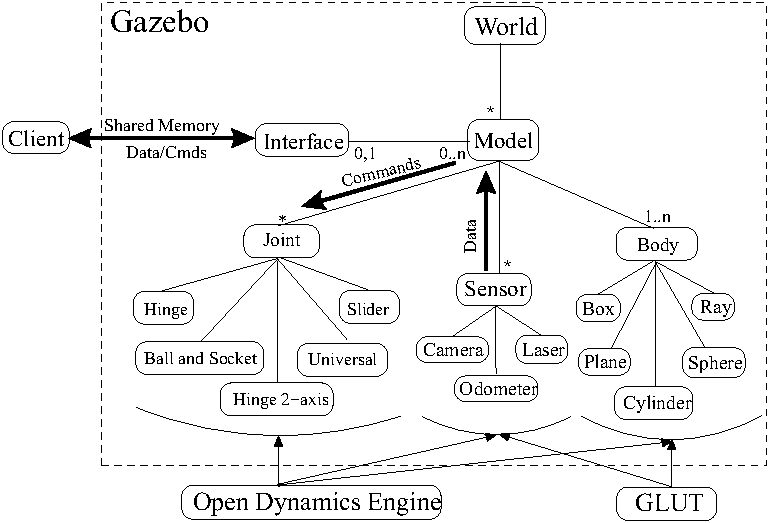
\includegraphics[height=8cm]{kapitel2/gazebo}
  \caption{Architektur des Gazebo-Frameworks \autocite{Koenig-2004-394}}
  \label{Kap2:gazeboarchitektur}
\end{figure}

\subsubsection{Physik-Engine}

Als Physik-Engine wird standardmäßig die \ac{ODE} genutzt. Es sind auch weitere Physik-Engines möglich, da diese nicht fest in der Architektur verdrahtet ist. Alternativ zum Standard können demnach Bullet, Simbody oder DART genutzt werden.
    
\subsubsection{Visualisierung}

Für die reine Visualisierung nutzt Gazebo standardmäßig OpenGL sowie GLUT (OpenGL Utility Toolkit). OpenGL ist plattformunabhängig, hochskalierbar, stabil und wird stetig weiterentwickelt. Außerdem sind viele Funktionalitäten in OpenGL auf Hardware-Ebene in der Grafikkarte entwickelt, so dass die CPU entlastet ist und andere Aufgaben schneller leisten kann.}

\subsubsection{Welt}

Die Gazebo-Welt ist eine Sammlung aus verschiedenen Komponenten:
\begin{itemize}
  \item \emph{Modelle}: Modelle sind Objekte mit einer physikalischen Definition.
  \item \emph{Körper}: Körper sind die grundlegenden geometrischen Bauteile beispielsweise des Roboters.
  \item \emph{Gelenke}: Gelenke verbinden die Körper miteinander und formen damit die möglichen kinematischen Bewegungen.
  \item \emph{Sensoren}: Ein Sensor in Gazebo ist ein abstraktes Gerät ohne physikalische Definition. Gazebo bietet aktuell  Odometriesensor, einen Nähesensor sowie eine Kamera an.
\end{itemize}
  
\subsubsection{Erstellung von Modellen}

Aktuell müssen Modelle per Hand erstellt werden. Dies erfolgt in der Regel über das sdf-Format. Kommt \ac{ROS} zum Einsatz, kann mittels der Node urdf\_spawner auch das urdf-Format verwendet werden.}
  
Abschließend ist noch wichtig, dass Gazebo durch Plugins erweiterbar ist und eine umfangreiche Schnittstelle bietet, die in einer \ac{ROS}-Node mit C++ oder Python aufgerufen werden kann. Des Weiteren lässt Gazebo auch ein Rendering der Simulation auf einem Remote-Server zu, so dass verteilte Anwendungen möglich werden. Dies ist in vielen Fällen aufgrund begrenzter Rechenleistung sehr von Vorteil. 